\documentclass[../DS07.tex]{subfiles}
\graphicspath{{./figures/}}

% \subimport{/home/nora/Documents/Enseignement/Prepa/bpep/exercices/DS/metronome/}{sujet.tex}

\begin{document}
\exercice[20]{Oscillations d'un métronome}

\enonce{
	\noindent
	\begin{minipage}[c]{.50\linewidth}
		On étudie un métronome constitué~:
		\begin{itemize}
			\item d'une tige rigide de longueur $L =\SI{20}{cm}$ de masse
			      négligeable en rotation d'angle $\th$ autour de l'axe $\Or z$~;
			\item d'un disque homogène de centre C, tel que $\mathrm{OC} = \ell =
				      \SI{2}{cm}$, de rayon $R = \SI{1,5}{cm}$ et de masse
			      $M = \SI{200}{g}$~;
			\item d'un curseur (dimensions négligeables) et de masse $m =
				      \SI{20}{g}$ et pouvant être déplacé sur la tige selon le rythme
			      souhaité. On appelle $x$ la distance du curseur à O, cette distance ne
			      pouvant dépasser $\SI{15}{cm}$.
		\end{itemize}
		La tige est tenue en $O$ par une liaison pivot supposée parfaite. On associe
		au bâti fixe le repère orthonormé ($O$, $\ux$, $\uy$, $\uz$). On
		donne le moment d'inertie par rapport à l'axe de rotation $\Or z$, orienté selon
		le vecteur $\uz$~:
		\[
			J = mx^ 2 + \frac{2}{5} MR^ 2 + M \ell ^ 2
		\]
	\end{minipage}
	\hfill
	\begin{minipage}[c]{.50\linewidth}
		\vspace{0pt}
		\begin{center}
			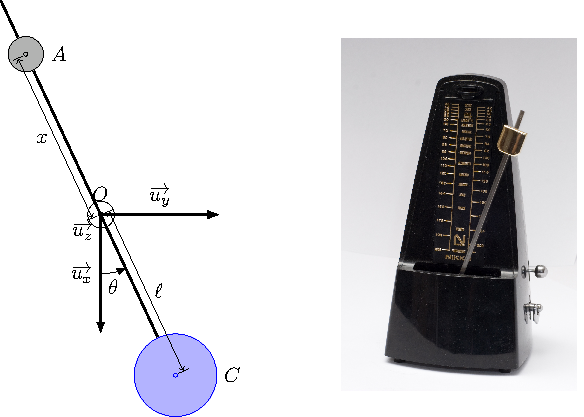
\includegraphics[width=\linewidth]{metronome.pdf}
			\captionof{figure}{%
				Schéma du métronome à gauche et photo d'un métronome (d'après wikipedia).
				Sur la photo, le contrepoids (disque homogène) n'est pas visible, seuls la
				tige et le curseur le sont.
			}
		\end{center}
	\end{minipage}
}%

\QR[2]{%
	Commenter et justifier l'influence de $x$ sur la valeur de $J$.
}{%
	Plus $x$ augmente et plus $J$ augmente \pt{1}, ce qui est normal puisque le
	moment d'inertie est d'autant plus grand que la masse est répartie loin de
	l'axe. \pt{1}
}%

% \QR{%
% 	Donner l'expression du moment cinétique $\Lc_{z}$ du métronome par rapport à
% 	l'axe $Oz$ en fonction des variables du problème.
% }{%
% 	\[
% 		\boxed{\Lc_{z} = J \tp}
% 	\]
% }%

\QR[8]{%
	Établir le système, faire un schéma puis le bilan des forces agissant sur le
	système et déterminer leurs moments par rapport à l'axe $\Or z$ par
	l'utilisation du \textbf{bras de levier}. Donnez l'expression du moment
	cinétique du système en fonction des données du problème.
}{%
	\noindent
	\begin{minipage}[t]{.75\linewidth}
		\begin{itemize}
			\bitem{Système}~: \{métronome\} = \{disque+tige+curseur\} de moment
			d'inertie $J_z$~;
			\bitem{Référentiel}~: terrestre supposé galiléen~;
			\hspace{100pt} \pt{1}
			\bitem{Repère}~: cylindrique $(\Or, \ur, \ut, \uz)$~;
			\bitem{Repérage}~: $\vvr{OC} = \ell \ur$ et $\vvr{OA} = -x\ur$.
			\hspace{100pt}
			\pt{1}
		\end{itemize}
		Les actions qui s'exercent sur le métronome sont~:
		\begin{itemize}
			\item poids du disque $\Pf\ind{C}  = M\gf$ dont le moment est
			      $\Mc _{z} (\Pf\ind{C}) = -Mg \ell\sin\th$~;
			      \hspace{10pt}
			      \pt{1}
			\item poids du curseur $\Pf\ind{A}  = m\gf $ dont le moment est
			      $\Mc _{z} (\Pf\ind{A}) = +mgx\sin\th$~;
			      \hspace{10pt}
			      \pt{1}
			\item liaison pivot parfaite dont le moment par rapport à l'axe $\Or z$ est
			      nul.
			      \hspace{10pt}
			      \pt{1}
			\item De plus, $\Lc_z(\Sc) = J \tp$.
			      \hspace{10pt}
			      \pt{1}
		\end{itemize}
	\end{minipage}
	\hfill
	\begin{minipage}[t]{.20\linewidth}
		\vspace{-15pt}
		\begin{center}
			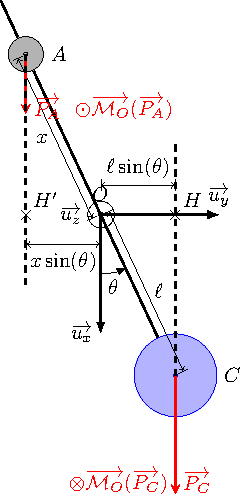
\includegraphics[width=.8\linewidth]{metronome_cor}
			\captionof{figure}{Schéma \protect \pt{2}}
		\end{center}
	\end{minipage}
	\hspace*{\fill}
}%

\QR[2]{%
	Déterminer l'équation différentielle du mouvement vérifiée par l'angle
	$\th$.
}{%
	On applique la loi du moment cinétique dans le référentiel galiléen du
	laboratoire~:
	\begin{gather*}
		\dv{\Lc_z}{t} \stm{=} \Mc_z(\Ff\ind{ext})
		\Lra
		J\tpp = mgx\sin\th-Mg \ell\sin\th
		\quad \Lra \quad
		\boxed{\tpp + \frac{Mg \ell - mgx}{J} \sin\th \stm{=} 0}
	\end{gather*}
}%

\QR[4]{%
	Dans l'hypothèse des petites oscillations, donner l'équation différentielle
	puis l'expression de la période propre $T_0$ des oscillations en fonction de
	$m$, $M$, $\ell$, $R$, $x$ et $g$
}{%
	Si les oscillations sont petites, alors $\sin\th\approx\th$, donc on
	retrouve l'équation différentielle de l'oscillateur harmonique~:
	\begin{gather*}
		\tpp + \frac{Mg \ell-mgx}{J}tp = 0
		\Lra
		\boxed{\tpp + \w_0{}^2tp \stm{=} 0}
		\\\Ra
		\w_0 \stm{=} \sqrt{\frac{Mg \ell - mgx}{J}}
		\Lra
		T_0 \stm{=} 2\pi \sqrt{\frac{J}{Mg \ell - mgx}}
		\Lra
		\boxed{T_0 \stm{=}
			2\pi \sqrt{\frac{mx^ 2 + \frac{2}{5} MR^ 2 + M \ell ^ 2}{Mg \ell - mgx}}}
	\end{gather*}
}%

% \begin{pycode}
% import numpy as np
% m = 20e-3  # kg
% M = 200e-3 # kg
% g = 10     # m.s^-2
% R = 1.5e-2 # m
% ell = 2e-2 # m
% T0 = 1.2   # s
% D = m**2*g*T0**2/(16*np.pi**4) - 4*m*(2/5*M*R**2 + M*ell**2 -
%     T0**2*M*g*ell/(4*np.pi**2))
%
% xp = -0.5*g*T0**2/(4*np.pi**2) + np.sqrt(D)/(2*m) # m
% xp = xp*1e2 # cm
% xm = -0.5*g*T0**2/(4*np.pi**2) - np.sqrt(D)/(2*m)
% xm = xm*1e2
% \end{pycode}

\QR[2]{%
	Dans une partition musicale le rythme est donné en battements par minute,
	c'est à dire le nombre de demis aller-retour du métronome. On a ainsi le
	mouvement \textit{andante} de \num{100} battements par minute. À quelle
	période du métronome correspondent ce mouvement~?
	% Calculer alors la distance
	% $x$ du curseur correspondant à ce \textit{tempo}, sans chercher son expression
	% littérale complète.
}{%
	Cela correspond à 50 périodes par minute \pt{1}, donc
	\begin{gather*}
		\boxed{
		T_0 =
		\frac{\SI{60}{s.min^{-1}}}{\SI{50}{\text{périodes}.min{^{-1}}}} =
		\SI{1,2}{s.\text{période}^{-1}} \pt{1}
		}
		% \\\beforetext{Ainsi}
		%   \frac{T_0{}^2}{4\pi^2} \left( Mg \ell - mgx \right) =
		%   mx^2 + \frac{2}{5}MR^2 + L \ell^2
		%   \\\Lra
		%   mx^2 + \frac{mg T_0{}^2}{4\pi^2}x + \frac{2}{5}MR^2 + M \ell^2 -
		%   \frac{T_0{}^2}{4\pi^2}Mg \ell = 0
		%   \\\Ra 
		%   \Delta = \frac{m^2g^2T_0{}^4}{16\pi^2} -
		%   4m\left(\frac{2}{5}MR^2 + M \ell^2 - \frac{T_0{}^2}{4\pi^2}Mg \ell\right)
		%   \\\Ra 
		%   \boxed{
		%     x = -\frac{gT_0{}^2}{8\pi^2} + \sqrt{\frac{\Delta}{4m^2}}
		%   }
		%   \Ra 
		%   \xul{x\ind{andante} = \SI{8.29}{cm}}%\py{fr'\SI{{{xp:.2f}}}{{cm}}'}}
	\end{gather*}
}%

\QR[2]{%
	Dans quel sens faut-il modifier $x$ pour augmenter le nombre de battements par
	minute pour un mouvement \textit{allegro} de \num{120} battements par
	minutes~?
}{%
	Pour augmenter la fréquence, il faut diminuer $T_0$, \pt{1} donc diminuer son
	numérateur et augmenter son dénominateur, ce qui revient dans les 2 cas à
	diminuer $x$. \pt{1}
}%

\end{document}
